\part{Appendices}

\chapter{Appendices for Chapter \ref{chap:comp}}

\section{Selected hyperparameters for the classifiers and the baseline}
\label{app:comp:sec:selectedhyperparameters}

When we train a classifier on extracted features, we tune its hyperparameters by cross-validation. For SVM, we tune the penalty parameter $C$ with values taken in 
$\left\{10^{-10}, 10^{-9},...,10\right\}$. For extremely randomized trees, we grow fully expanded trees and tune the number of features evaluated at each split $k$ among $\left\{1, \sqrt{n_f}, \frac{n_f}{2}, n_f\right\}$ where 
$n_f$ is the total number of features. For the single layer perceptron, we tune the number of iterations among $\left\{1000, 2500, 5000, 10000\right\}$ and the learning rate among $\left\{10^{-4}, 10^{-3}, 10^{-2}, 10^{-1}\right\}$. All the other parameters values are the ones provided by default by the scikit-learn package \parencite{scikit-learn}. More precisely, we use: the Adam \parencite{kingma2014adam} optimizer with default parameters, an L2 penalty on the weights with $\alpha$ set to $10^{-4}$ and a batch size of 200 samples.

For the baseline ET-FL, we tune the size of the windows $\left(w_{min}, w_{max}\right)$ among all valid size ranges with \texttt{min\_size} in $\left\{0.0, 0.25, 0.5, 0.75\right\}$ and \texttt{max\_size} in $\left\{0.25, 0.5, 0.75, 1.0\right\}$ and the colorspace $L$ among $\left\{\texttt{TRGB}, \texttt{HSV}\right\}$ where \texttt{TRGB} and \texttt{HSV} are respectively the normalized RGB and hue-saturation-value colorspaces. The number of extracted subwindow per image $w$ is taken such that the total number of subwindows for the dataset $w_t$ is approximately 1 million. The other fixed parameters are $T$, the number of trees, $l_{min}$, the minimum number of samples in a leave of a tree. The value for those parameters as well as the selected values for tuned parameters are given in Table \ref{app:comp:tab:hyper_etfl}. 

\begin{table}
	\centering
	\begin{tabular}{|c|c|c|c|c|c|c|c|c|c|}
    	\hline
        \multirow{2}{*}{\textbf{Datasets}} & \multicolumn{6}{c|}{Fixed} & \multicolumn{3}{c|}{Tuned (best)} \\ 
     	\cline{2-10}
		 & $T$ & $w$ & $w_t$ & $l_{min}$ & $k$ & $C$ & $w_{min}$ & $w_{max}$ & $L$ \\ 
     	\hline
        C & 20 &  551 & 1000616 & 1000 & 384 & 0.01 & 0.25 & 0.50 & TRGB \\
        G & 20 &   69 & 1007745 & 1000 & 384 & 0.01 & 0.00 & 0.75 &  HSV \\
        P & 20 &  743 & 1000078 & 1000 & 384 & 0.01 & 0.25 & 0.50 &  HSV \\
        N & 20 & 1265 & 1000615 & 1000 & 384 & 0.01 & 0.00 & 0.25 &  HSV \\
        B & 20 &   55 & 1004355 & 1000 & 384 & 0.01 & 0.00 & 0.75 &  HSV \\
        M & 20 &  261 & 1001457 & 1000 & 384 & 0.01 & 0.25 & 0.75 & TRGB \\
        L & 20 &  184 & 1001512 & 1000 & 384 & 0.01 & 0.25 & 0.50 &  HSV \\
        H & 20 &  228 & 1002516 & 1000 & 384 & 0.01 & 0.25 & 0.50 & TRGB \\
     	\hline
	\end{tabular}
    \caption{Hyperparameters for ET-FL.}
    \label{app:comp:tab:hyper_etfl}
\end{table}

\section{Best features}
\label{app:comp:sec:bestfeatures}

In order to investigate the best features (according to feature importances) for a given network, we compute the minimum size of the best features subset so that at least one feature is in this subset for all datasets. The resulting sizes for all networks are given in Table \ref{app:comp:tab:best_subset_size}. We also compute the percentages of overlap between subsets of selected features by RFE for all pairs of datasets (see Table \ref{app:comp:tab:rfe_sub_overlap})

\begin{table}
\centering
\begin{tabular}{|c|cc|}
\hline
$\mathcal{N}$ & \textbf{\# feat.} & \textbf{\% feat.} \\
\hline
Mobile & 753 & 73.54 \\
IncResV2 & 1277 & 83.14 \\
IncV3 & 1537 & 75.05 \\
ResNet & 1803 & 88.04 \\
VGG16 & 409 & 79.88 \\
VGG19 & 392 & 76.56 \\
DenseNet & 1477 & 76.93 \\
\hline
\end{tabular}
\caption{Given a network, this table gives the best features subset minimum size so that there is at least one feature that is in this subset for all datasets.}
\label{app:comp:tab:best_subset_size}
\end{table}

\section{Features and cut points information}
\label{app:comp:sec:features_and_cut_points}

In the paper, we investigate the usage of features from inside the networks. Therefore, we have selected the layers from which we would extract the features. As stated in the paper, we limit the number of possible cut points to the bottlenecks of the networks, a bottleneck being a point were several paths are merged into a single one. For ResNet, we have selected the ReLU activations of the merging layer after each residual block. 
For IncResV2, considering all the bottlenecks after inception-resnet and reduction blocks yields approximately fifty possible cut points, that is more than 100k features. We have decided to subsample those cut points to obtain a number of features closer to those of other networks while covering the network as uniformly as possible along its depth. As far as DenseNet is concerned, we extract features only at the end of dense blocks and after pooling blocks. Indeed, extracting features inside dense blocks would have resulted in duplicated features.  

In Table \ref{app:comp:tab:n_features_per_net} are given the information about the generated features vectors for the ``\textit{Last layer}", ``\textit{Merging features across networks}" and ``\textit{Merging layers features}" experiments. Information about the dimensions of the extracted features from inside the networks (before global average pooling) for ResNet, IncResV2 and DenseNet are respectively given in Tables \ref{app:comp:tab:inner_layers_resnet}, \ref{app:comp:tab:inner_layers_incresv2} and \ref{app:comp:tab:inner_layers_densenet}. The layer names given in those tables are the the ones given by the Keras package \parencite{chollet2015keras}. 

 \begin{table}
     \center 
     \begin{tabular}{|c|c|c|c|}
         \hline
         \multirow{2}{*}{$\mathcal{N}$} & \multicolumn{1}{c|}{\textbf{Last layer}} & \multicolumn{2}{c|}{\textbf{Merged layers}} \\
         \cline{2-4}
         & \# feat. & \# feat. & \# cut \\
         \hline
         Mobile & 1024 & / & /\\ 
         DenseNet & 1920 & 7744 & 9 \\ 
         IncResV2 & 1536 & 17088 & 12 \\ 
         ResNet & 2048 & 15168 & 17 \\ 
%          IncV3 & 2048 & 10112 & 12 \\ 
         IncV3 & 2048 & / & / \\ 
         VGG19 & 512 & / & / \\ 
         VGG16 & 512 & / & / \\  
         \hline
         \textbf{Total} & 9600 & / & / \\
         \hline 
     \end{tabular}
     \caption{Number of features extracted for the ``\textit{Last layer}'' experiment. Total number of features for the ``\textit{Merging features across networks}". Number of features and cut points for the ``\textit{Mering layers features}'' experiment.}
     \label{app:comp:tab:n_features_per_net}
 \end{table}
 


\begin{table}
\centering
\begin{tabular}{|c|ccc|}
\hline
\multirow{2}{*}{\textbf{Layer $l$} (name)} & \multicolumn{3}{c|}{\textbf{Feat. maps dim.}}\\
& $h_a$ & $w_a$ & $d$ \\
\hline
activation\_1 & 112 & 112 & 64 \\
activation\_4 & 55 & 55 & 256 \\
activation\_7 & 55 & 55 & 256 \\
activation\_10 & 55 & 55 & 256 \\
activation\_13 & 28 & 28 & 512 \\
activation\_16 & 28 & 28 & 512 \\
activation\_19 & 28 & 28 & 512 \\
activation\_22 & 28 & 28 & 512 \\
activation\_25 & 14 & 14 & 1024 \\
activation\_28 & 14 & 14 & 1024 \\
activation\_31 & 14 & 14 & 1024 \\
activation\_34 & 14 & 14 & 1024 \\
activation\_37 & 14 & 14 & 1024 \\
activation\_40 & 14 & 14 & 1024 \\
activation\_43 & 7 & 7 & 2048 \\
activation\_46 & 7 & 7 & 2048 \\
activation\_49 (last) & 7 & 7 & 2048 \\
\hline
\textbf{Total} & / & / & \textbf{15168} \\
\hline 
\end{tabular}
\caption{Name and dimensions of the layers extracted from inside ResNet for the ``\textit{Merging features across layers}'' and ``\textit{Inner layers}'' experiments.}
\label{app:comp:tab:inner_layers_resnet}
\end{table}


\begin{table}
\centering
\begin{tabular}{|c|ccc|}
\hline
\multirow{2}{*}{\textbf{Layer $l$} (name)} & \multicolumn{3}{c|}{\textbf{Feat. maps dim.}}\\
& $h_a$ & $w_a$ & $d$ \\
\hline
max\_pooling2d\_2 & 25 & 25 & 192 \\
mixed\_5b & 25 & 25 & 320 \\
block35\_1\_ac & 25 & 25 & 320 \\
block35\_4\_ac & 25 & 25 & 320 \\
block35\_7\_ac & 25 & 25 & 320 \\
block35\_10\_ac & 25 & 25 & 320 \\
mixed\_6a & 12 & 12 & 1088 \\
block17\_5\_ac & 12 & 12 & 1088 \\
block17\_10\_ac & 12 & 12 & 1088 \\
block17\_15\_ac & 12 & 12 & 1088 \\
block17\_20\_ac & 12 & 12 & 1088 \\
mixed\_7a & 5 & 5 & 2080 \\
block8\_3\_ac & 5 & 5 & 2080 \\
block8\_6\_ac & 5 & 5 & 2080 \\
block8\_9\_ac & 5 & 5 & 2080 \\
conv\_7b\_ac (last) & 5 & 5 & 1536 \\
\hline
\textbf{Total} & / & / & \textbf{17088} \\
\hline 
\end{tabular}
\caption{Name and dimensions of the layers extracted from inside IncResV2 for the ``\textit{Merging features across layers}'' and ``\textit{Inner layers}'' experiments.}
\label{app:comp:tab:inner_layers_incresv2}
\end{table}


\begin{table}
\centering
\begin{tabular}{|c|ccc|}
\hline
\multirow{2}{*}{\textbf{Layer $l$} (name)} & \multicolumn{3}{c|}{\textbf{Feat. maps dim.}}\\
& $h_a$ & $w_a$ & $d$ \\
\hline
pool1 & 56 & 56 & 64 \\
conv2\_block6\_concat & 56 & 56 & 256 \\
pool2\_pool & 28 & 28 & 128 \\
conv3\_block12\_concat & 28 & 28 & 512 \\
pool3\_pool & 14 & 14 & 256 \\
conv4\_block48\_concat & 14 & 14 & 1792 \\
pool4\_pool & 7 & 7 & 896 \\
conv5\_block32\_concat & 7 & 7 & 1920 \\
bn (last)& 7 & 7 & 1920 \\
\hline
\textbf{Total} & / & / & \textbf{7744} \\
\hline 
\end{tabular}
\caption{Name and dimensions of the layers extracted from inside DenseNet for the ``\textit{Merging features across layers}'' and ``\textit{Inner layers}'' experiments.}
\label{app:comp:tab:inner_layers_densenet}
\end{table}


\section{Features selected with RFE}
\label{app:comp:sec:rfe_selection}
A summary of the number of selected features and the cross-validation curves for all datasets and networks are respectively given in Table \ref{app:comp:tab:rfe_selected} and FigureS \ref{app:comp:fig:rfe_1} and \ref{app:comp:fig:rfe_2}.

\begin{table}
     \center 
     \begin{tabular}{|c|cccccccc|}
         \hline
         \multirow{2}{*}{$\mathcal{N}$} & \multicolumn{8}{c|}{\textbf{Number of features}} \\
         \cline{2-9}
         & C & P & G & N & B & M & L & H \\ 
         \hline
         Mobile & 25 & 257 & 33 & 13 & 57 & 169 & 45 & 213 \\
         DenseNet & 25 & 37 & 17 & 13 & 49 & 241 & 57 & 245 \\
         IncResV2 & 29 & 53 & 29 & 13 & 185 & 249 & 69 & 173 \\
         ResNet & 13 & 69 & 33 & 97 & 57 & 89 & 77 & 109 \\
         IncV3 & 33 & 13 & 37 & 13 & 97 & 121 & 105 & 137 \\
         VGG19 & 25 & 41 & 41 & 21 & 25 & 161 & 61 & 73 \\
         VGG16 & 25 & 29 & 33 & 29 & 49 & 225 & 93 & 113 \\
         \hline
         
     \end{tabular}
     \caption{Number of features selected by RFE for all datasets and networks.}
     \label{app:comp:tab:rfe_selected}
 \end{table}
 
 \begin{table}
     \center 
     \begin{tabular}{|c|cccccccc|c|}
         \hline
         \multirow{2}{*}{$\mathcal{N}$} & \multicolumn{8}{c|}{\textbf{Proportion of features (\%)}} & \multirow{2}{*}{Average}\\
         \cline{2-9}
         & C & P & G & N & B & M & L & H & \\ 
         \hline
         Mobile & 2.44 & 25.10 & 3.22 & 1.27 & 5.57 & 16.50 & 4.39 & 20.80 & 9.91 \\
         DenseNet & 1.30 & 1.93 & 0.89 & 0.68 & 2.55 & 12.55 & 2.97 & 12.76 & 4.45 \\
         IncResV2 & 1.89 & 3.45 & 1.89 & 0.85 & 12.04 & 16.21 & 4.49 & 11.26 & 6.51 \\
         ResNet & 0.63 & 3.37 & 1.61 & 4.74 & 2.78 & 4.35 & 3.76 & 5.32 & 3.32 \\
         IncV3 & 1.61 & 0.63 & 1.81 & 0.63 & 4.74 & 5.91 & 5.13 & 6.69 & 3.39 \\
         VGG19 & 4.88 & 8.01 & 8.01 & 4.10 & 4.88 & 31.45 & 11.91 & 14.26 & 10.94 \\
         VGG16 & 4.88 & 5.66 & 6.45 & 5.66 & 9.57 & 43.95 & 18.16 & 22.07 & 14.55 \\
         \hline
         Average & 2.52 & 6.88 & 3.41 & 2.56 & 6.02 & 18.70 & 7.26 & 13.31 & \textbf{7.58} \\
         \hline
     \end{tabular}
     \caption{Proportion of features selected by RFE for all datasets and networks.}
     \label{app:comp:tab:rfe_selected_prop}
 \end{table}
 
 \section{Detailed scores for transfer learning experiments}
\label{app:comp:sec:detailed_scores}

Detailed scores for all datasets, experiments and networks are given in Tables \ref{app:comp:tab:detailed_first} and \ref{app:comp:tab:detailed_second}.

\begin{figure}
	\centering
  \begin{subfigure}{0.95\textwidth}
    \centering
    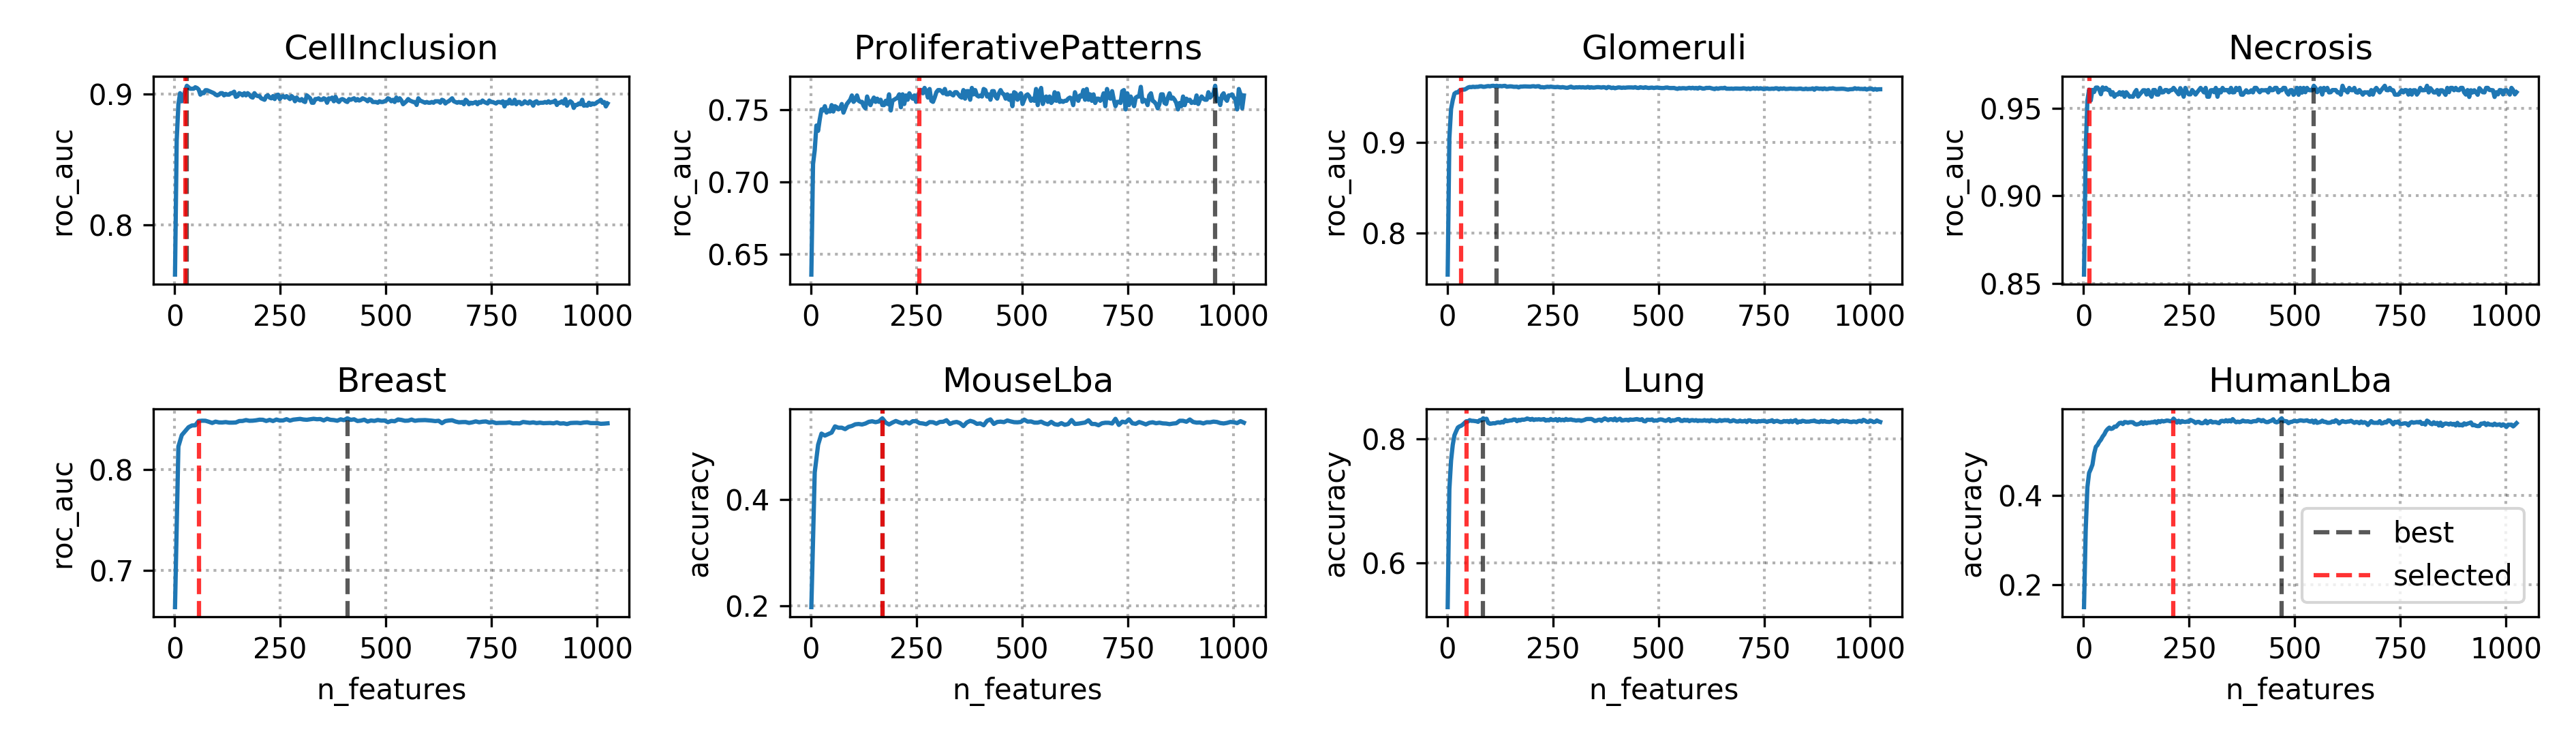
\includegraphics[width=\textwidth]{comp/supp/rfe_mobile.png} \\
    \caption{Mobile}
  \end{subfigure}
  \begin{subfigure}{0.95\textwidth}
    \centering
    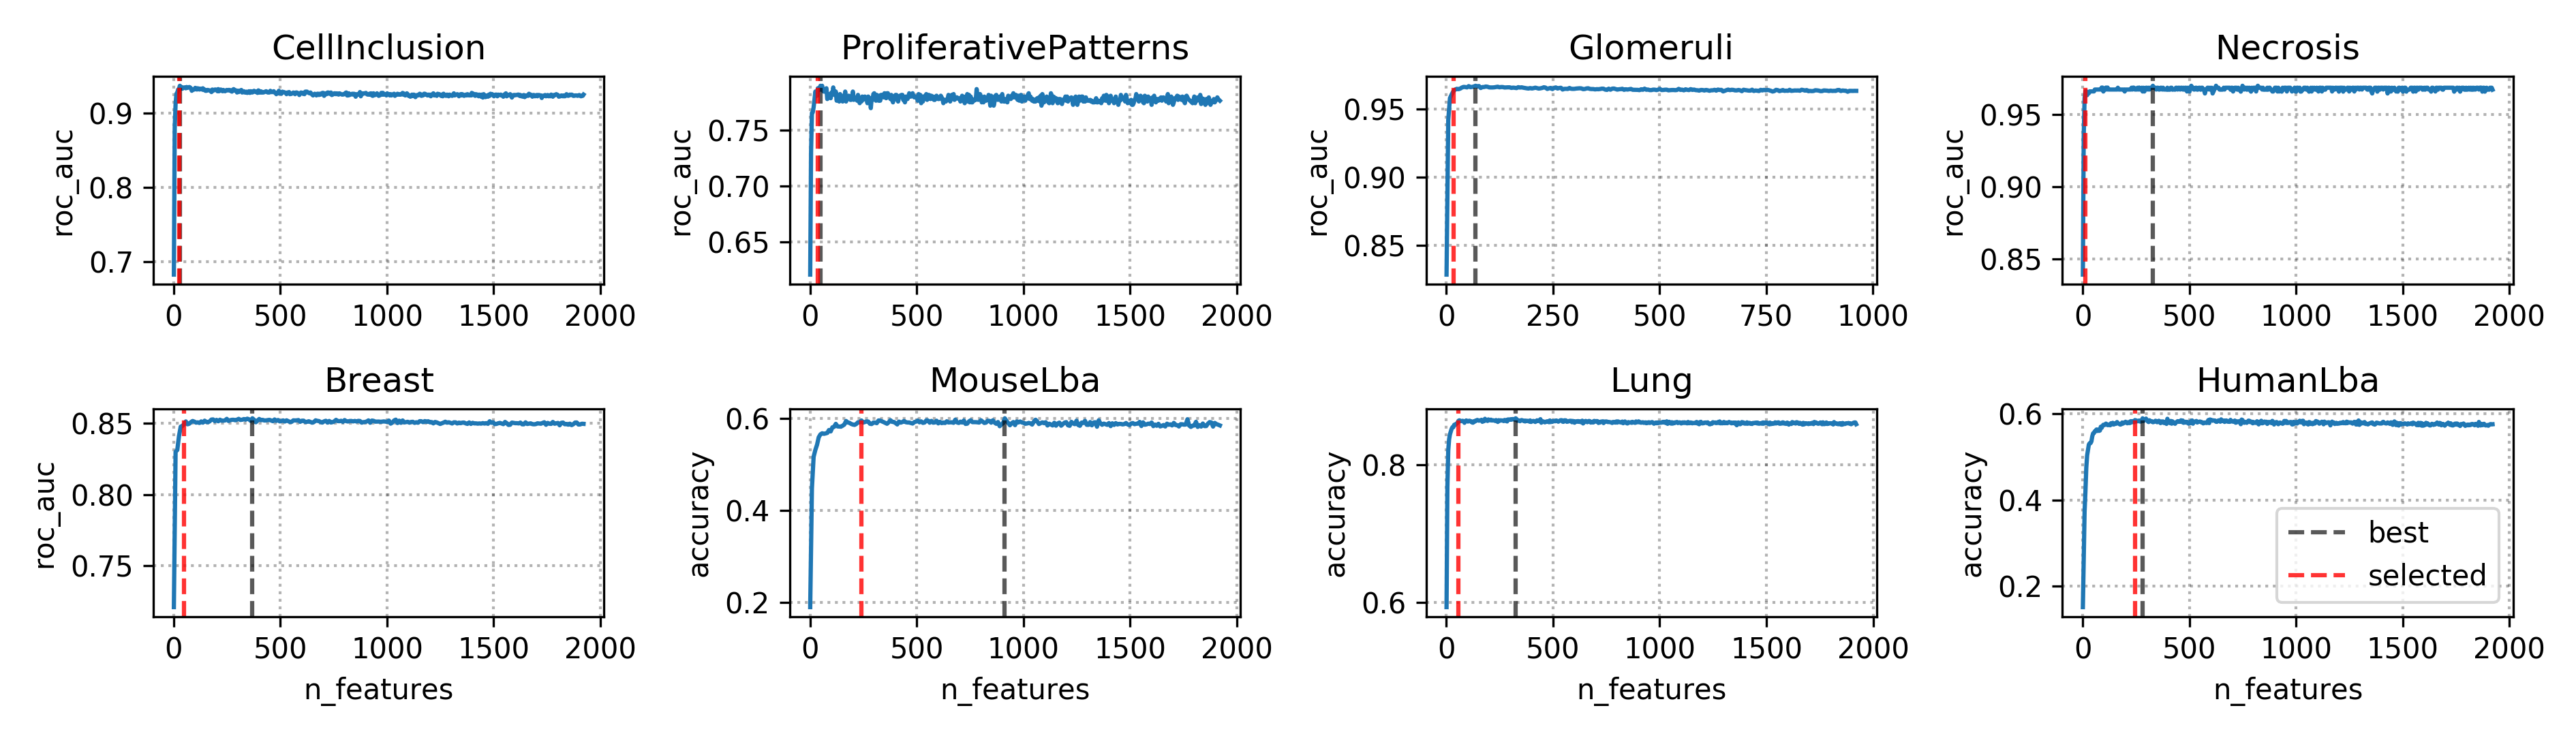
\includegraphics[width=\textwidth]{comp/supp/rfe_dense_net_201.png} \\
    \caption{DenseNet}
  \end{subfigure}
  \begin{subfigure}{0.95\textwidth}
    \centering
    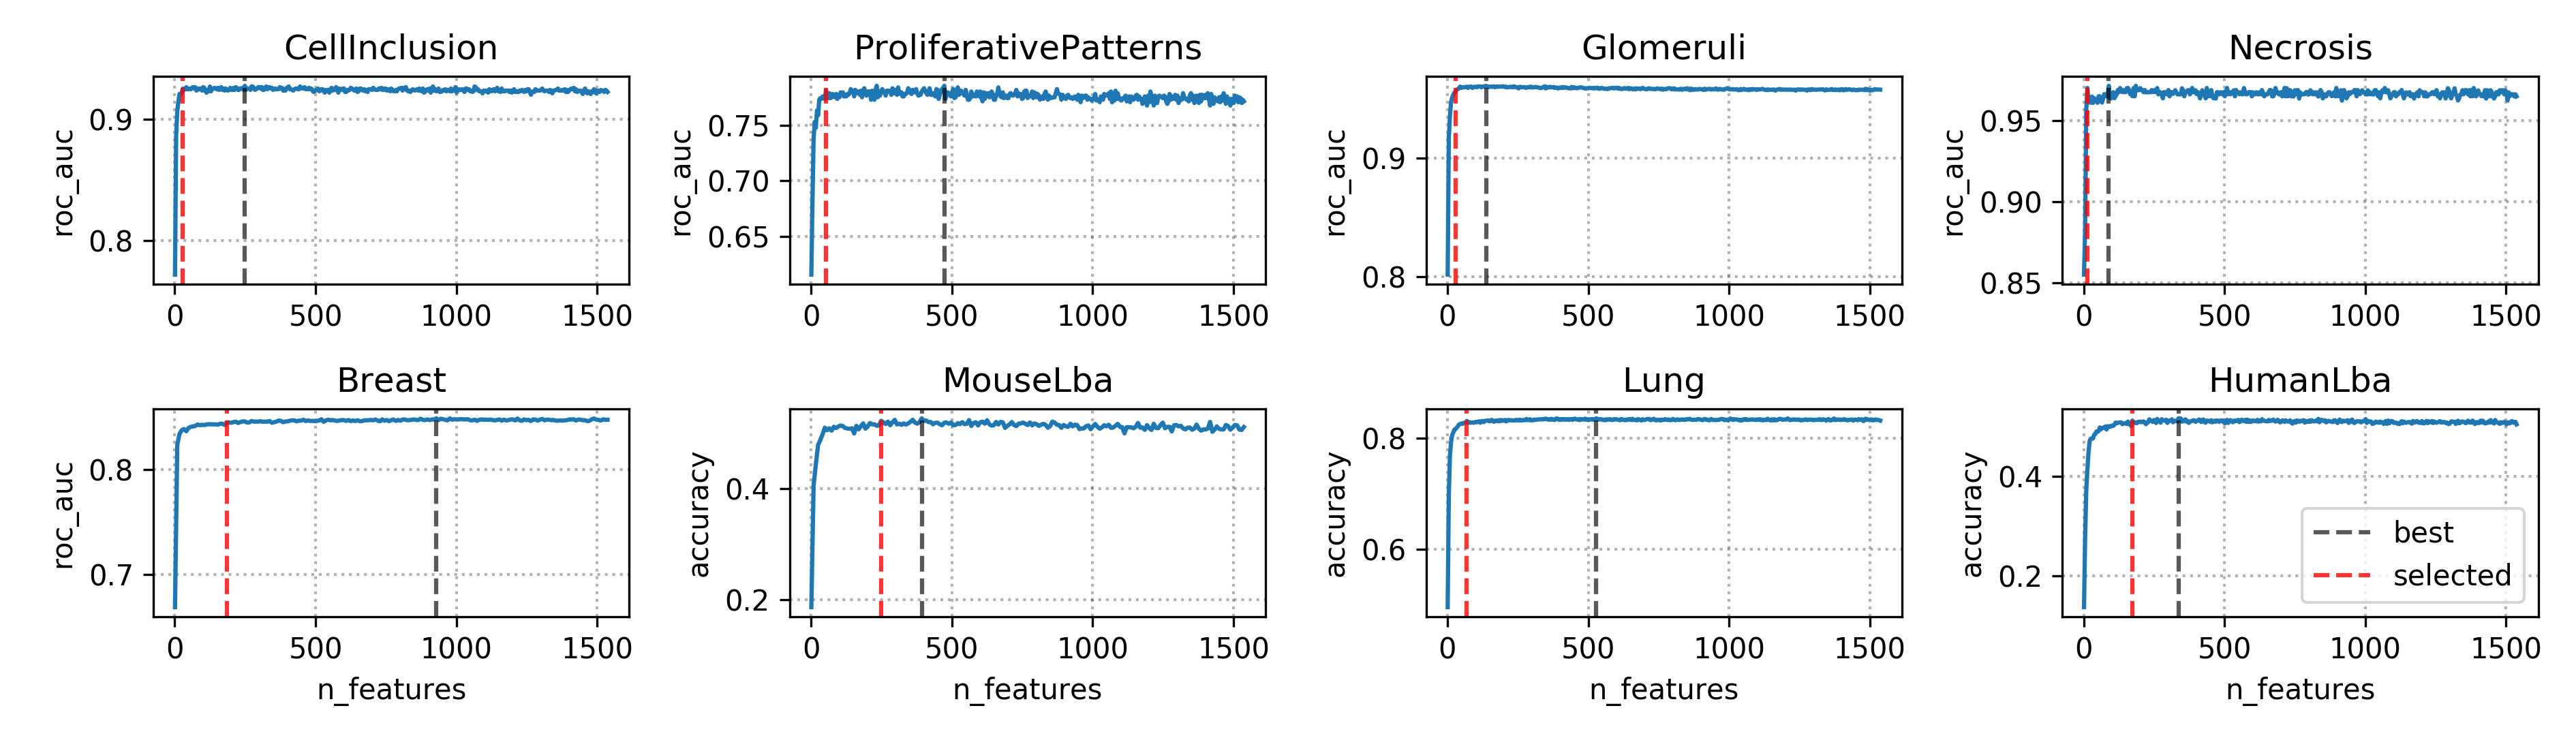
\includegraphics[width=\textwidth]{comp/supp/rfe_inception_resnet_v2.png} \\
    \caption{IncResV2}
  \end{subfigure}
    \begin{subfigure}{0.95\textwidth}
    \centering
    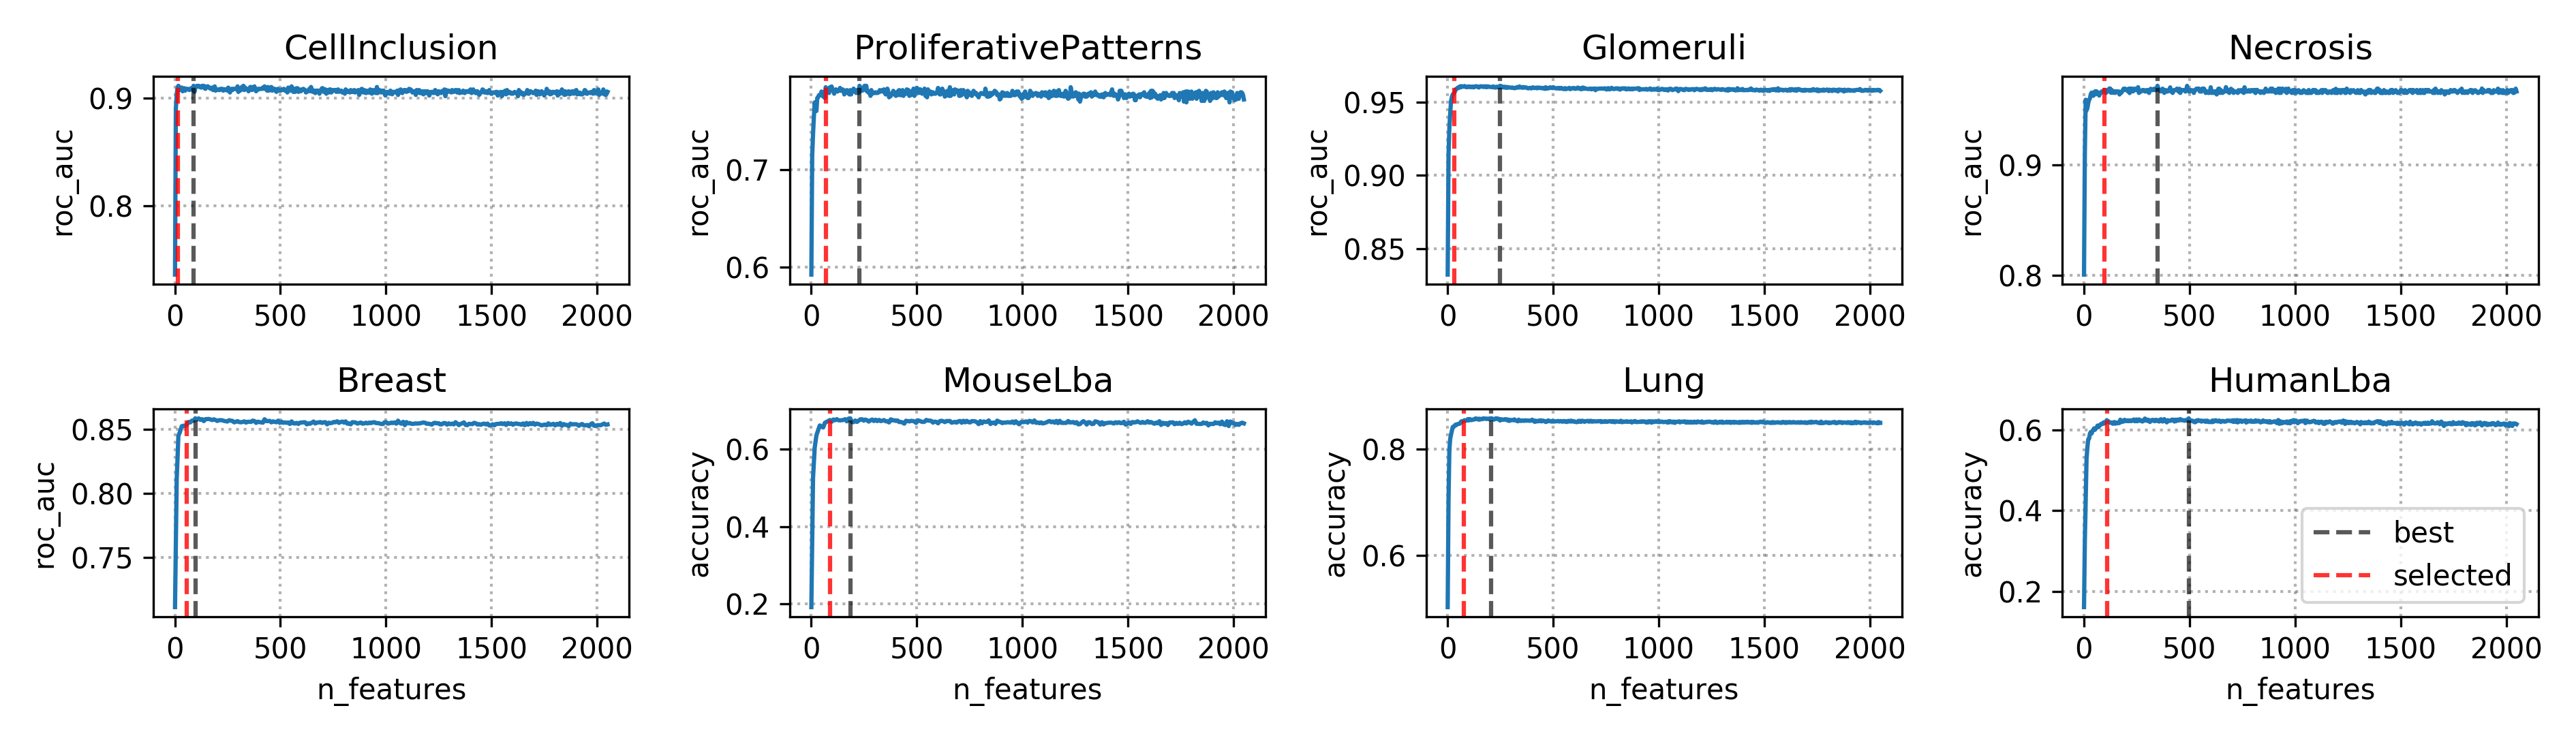
\includegraphics[width=\textwidth]{comp/supp/rfe_resnet50.png}
    \caption{ResNet}
  \end{subfigure}
  \caption{RFE curves for last layers features from InceptionV3, VGG19 and VGG16.}
  \label{app:comp:fig:rfe_1}
\end{figure}

\begin{figure}
	\centering
  \begin{subfigure}{0.95\textwidth}
    \centering
    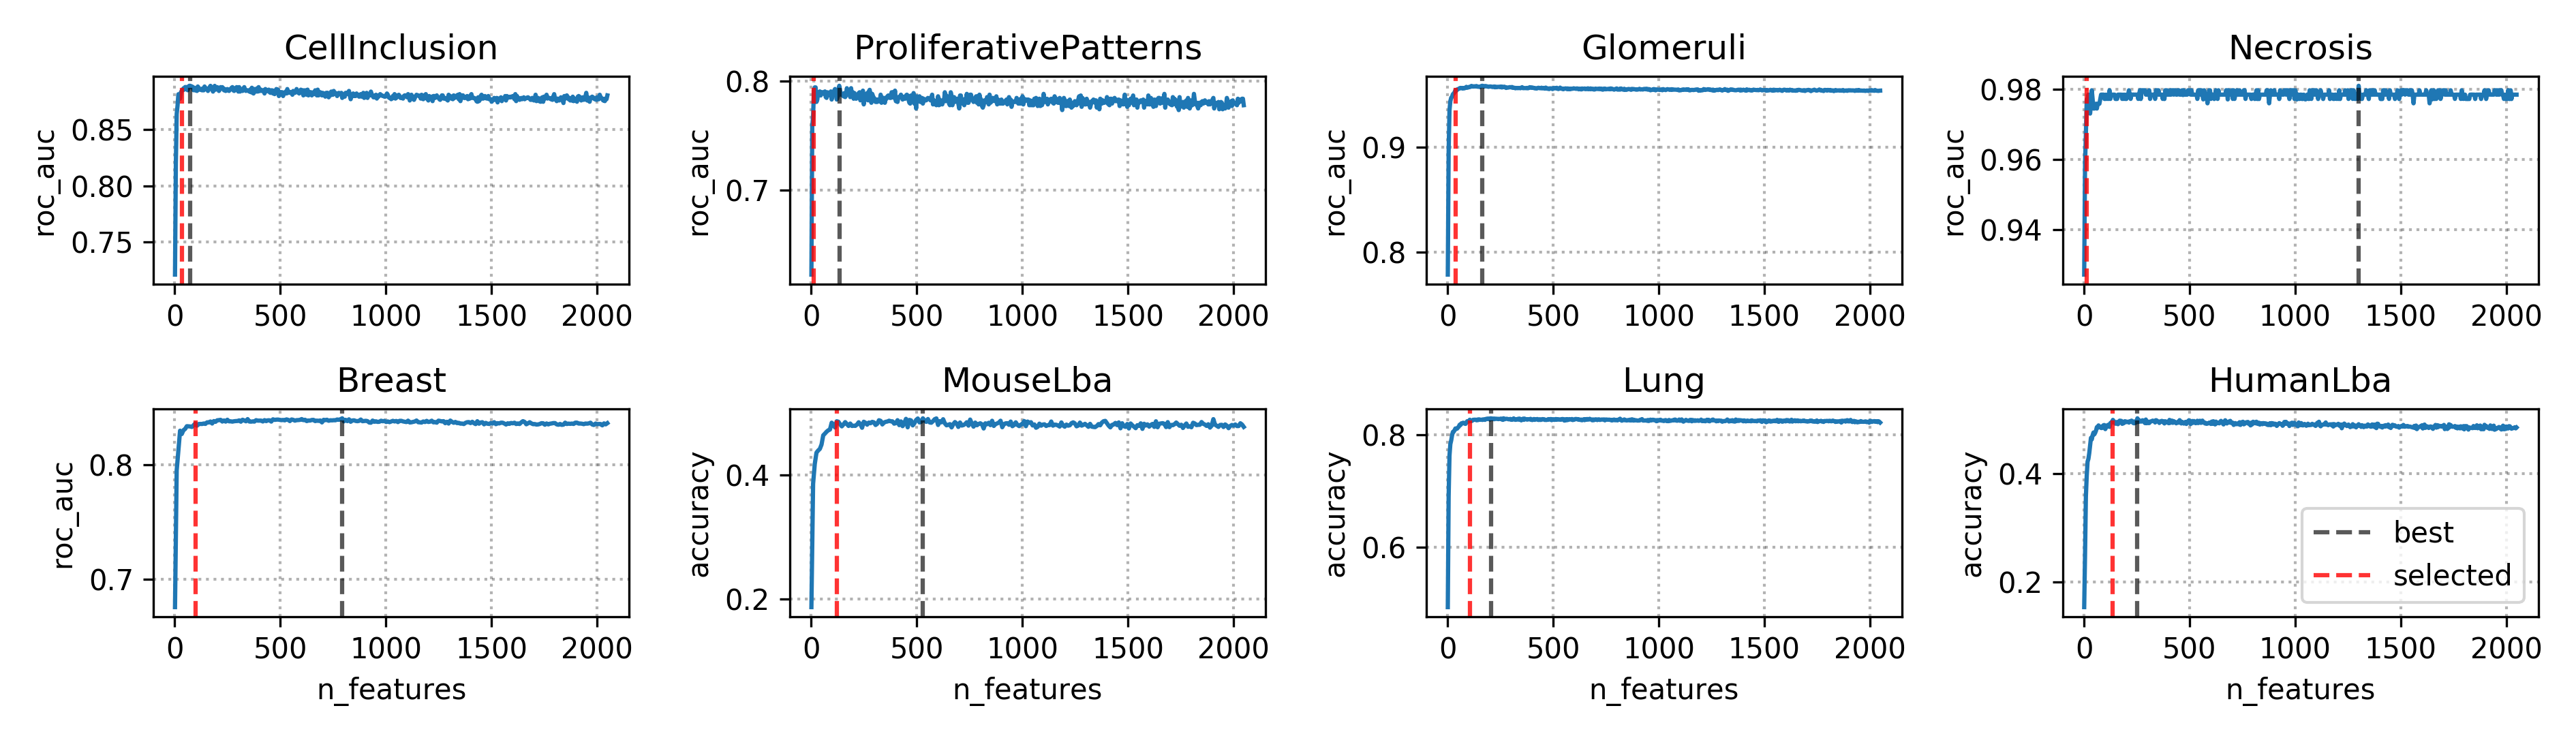
\includegraphics[width=\textwidth]{comp/supp/rfe_inception_v3.png} \\
    \caption{IncV3}
  \end{subfigure}
  \begin{subfigure}{0.95\textwidth}
    \centering
    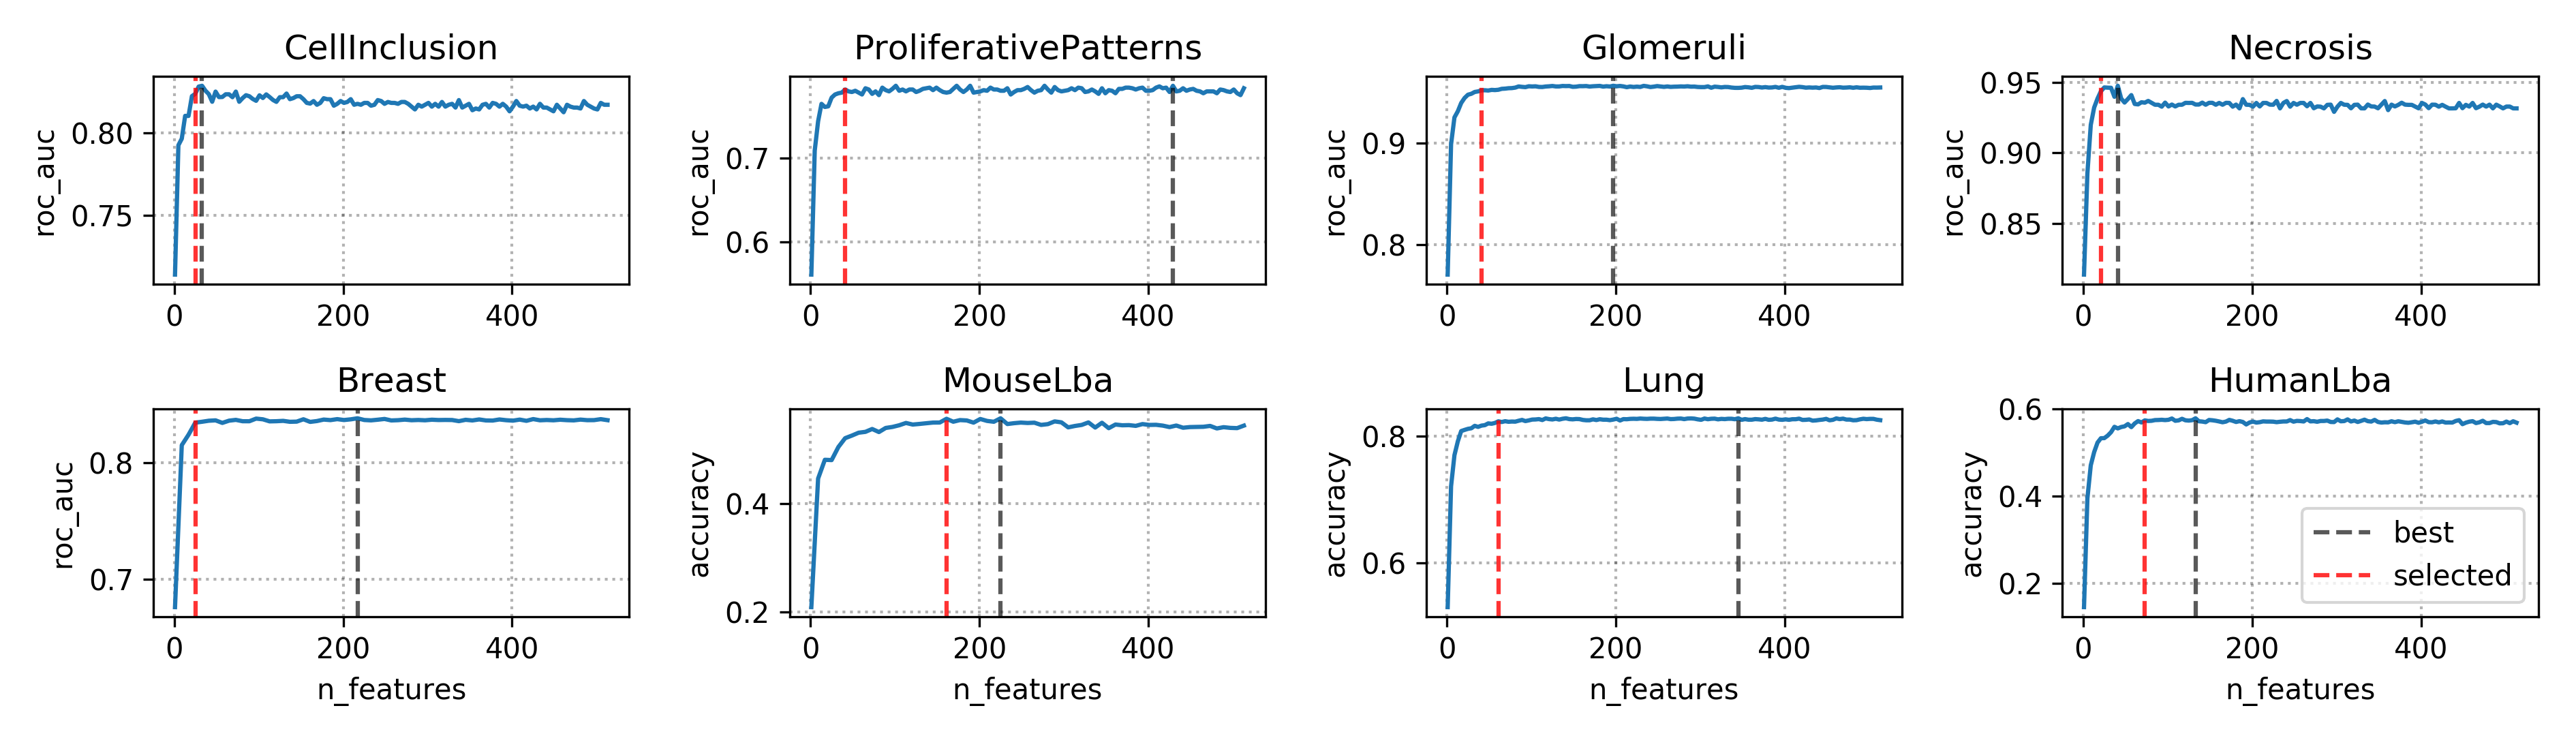
\includegraphics[width=\textwidth]{comp/supp/rfe_vgg19.png} \\
    \caption{VGG19}
  \end{subfigure}
  \begin{subfigure}{0.95\textwidth}
    \centering
    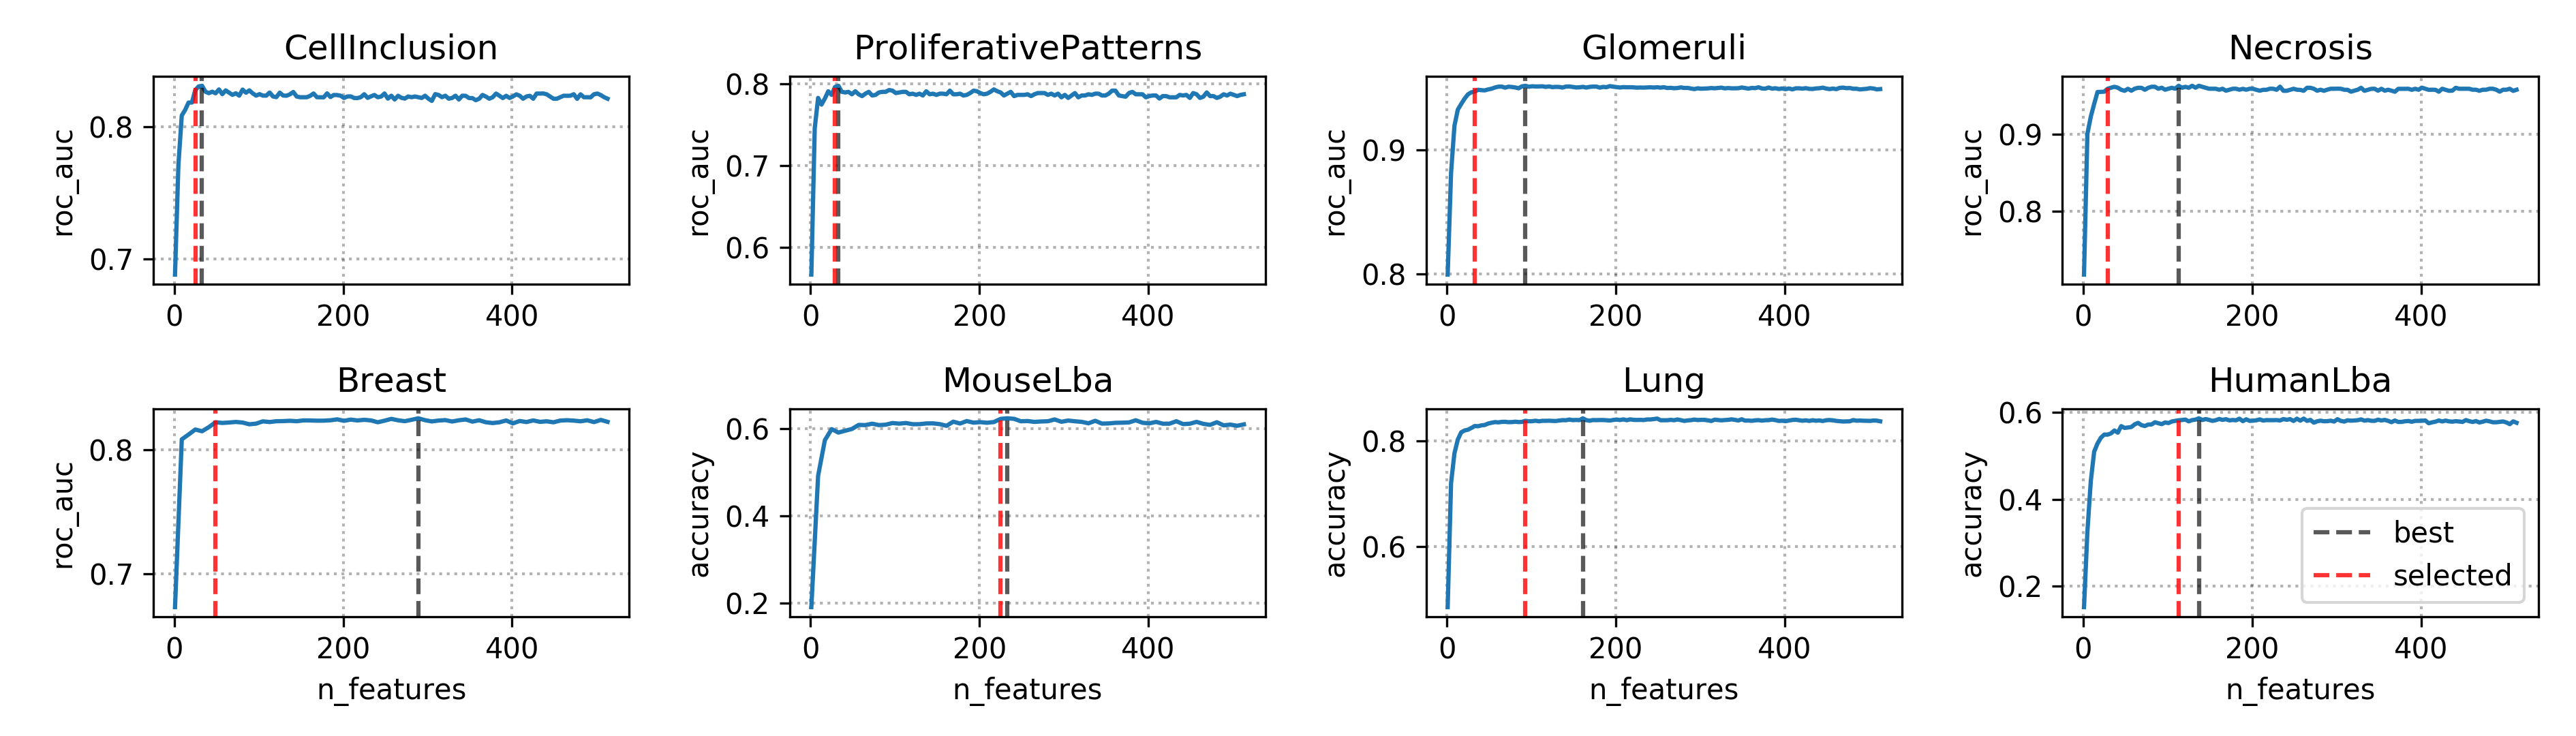
\includegraphics[width=\textwidth]{comp/supp/rfe_vgg16.png} \\
    \caption{VGG16}
  \end{subfigure}
  \caption{Cross validation curves from \acrlong{rfe} for last layers features from InceptionV3, VGG19 and VGG16.}
  \label{app:comp:fig:rfe_2}
\end{figure}

\begin{table}
  \centering
  \small
  \begin{subtable}{0.45\textwidth}
    \centering
    \begin{tabular}{|c|cccccccc|} 
    \hline
    Dataset & \textbf{C} & \textbf{P} & \textbf{G} & \textbf{N} & \textbf{B} & \textbf{M} & \textbf{L} & \textbf{H}\\
    \hline
    \textbf{C} &   & 1 & 3 & 0 & 0 & 3 & 4 & 2 \\
    \textbf{P} & 20 &   & 27 & 53 & 40 & 33 & 33 & 34 \\
    \textbf{G} & 4 & 3 &   & 7 & 14 & 4 & 15 & 6 \\
    \textbf{N} & 0 & 2 & 3 &   & 5 & 1 & 4 & 0 \\
    \textbf{B} & 0 & 8 & 24 & 23 &   & 5 & 17 & 8 \\
    \textbf{M} & 24 & 22 & 21 & 15 & 17 &   & 26 & 31 \\
    \textbf{L} & 8 & 5 & 21 & 15 & 14 & 7 &   & 6 \\
    \textbf{H} & 20 & 28 & 39 & 15 & 33 & 40 & 31 & \\
    \hline
    \end{tabular}
    \caption{Mobile}
  \end{subtable}

  \begin{subtable}{0.45\textwidth}
    \centering
    \begin{tabular}{|c|cccccccc|} 
    \hline
    Dataset & \textbf{C} & \textbf{P} & \textbf{G} & \textbf{N} & \textbf{B} & \textbf{M} & \textbf{L} & \textbf{H}\\
    \hline
    \textbf{C} &   & 1 & 0 & 0 & 3 & 2 & 7 & 3 \\
    \textbf{P} & 3 &   & 3 & 0 & 6 & 4 & 2 & 5 \\
    \textbf{G} & 0 & 1 &   & 0 & 1 & 2 & 0 & 1 \\
    \textbf{N} & 0 & 0 & 0 &   & 0 & 0 & 0 & 0 \\
    \textbf{B} & 20 & 22 & 10 & 7 &   & 14 & 20 & 13 \\
    \textbf{M} & 17 & 22 & 17 & 15 & 18 &   & 20 & 21 \\
    \textbf{L} & 17 & 3 & 0 & 0 & 7 & 5 &   & 7 \\
    \textbf{H} & 20 & 17 & 10 & 0 & 12 & 14 & 18 & \\
    \hline
    \end{tabular}
    \caption{IncResV2}
  \end{subtable}

  \begin{subtable}{0.45\textwidth}
    \centering
    \begin{tabular}{|c|cccccccc|} 
    \hline
    Dataset & \textbf{C} & \textbf{P} & \textbf{G} & \textbf{N} & \textbf{B} & \textbf{M} & \textbf{L} & \textbf{H}\\
    \hline
    \textbf{C} &   & 0 & 2 & 0 & 4 & 2 & 3 & 3 \\
    \textbf{P} & 0 &   & 0 & 7 & 0 & 1 & 2 & 1 \\
    \textbf{G} & 3 & 0 &   & 0 & 8 & 1 & 6 & 0 \\
    \textbf{N} & 0 & 7 & 0 &   & 2 & 2 & 1 & 1 \\
    \textbf{B} & 12 & 0 & 21 & 15 &   & 10 & 13 & 10 \\
    \textbf{M} & 9 & 15 & 5 & 23 & 13 &   & 21 & 20 \\
    \textbf{L} & 12 & 23 & 18 & 15 & 14 & 19 &   & 10 \\
    \textbf{H} & 15 & 15 & 2 & 15 & 15 & 23 & 14 & \\
    \hline
    \end{tabular}
    \caption{IncV3}
  \end{subtable}

  \begin{subtable}{0.45\textwidth}
    \centering
    \begin{tabular}{|c|cccccccc|} 
    \hline
    Dataset & \textbf{C} & \textbf{P} & \textbf{G} & \textbf{N} & \textbf{B} & \textbf{M} & \textbf{L} & \textbf{H}\\
    \hline
    \textbf{C} &   & 2 & 0 & 2 & 3 & 3 & 0 & 2 \\
    \textbf{P} & 15 &   & 0 & 7 & 7 & 7 & 14 & 11 \\
    \textbf{G} & 0 & 0 &   & 2 & 5 & 2 & 5 & 1 \\
    \textbf{N} & 15 & 10 & 6 &   & 19 & 11 & 11 & 9 \\
    \textbf{B} & 15 & 5 & 9 & 11 &   & 6 & 16 & 11 \\
    \textbf{M} & 23 & 10 & 6 & 10 & 10 &   & 10 & 23 \\
    \textbf{L} & 0 & 15 & 12 & 9 & 22 & 9 &   & 10 \\
    \textbf{H} & 23 & 18 & 6 & 10 & 21 & 29 & 14 & \\
    \hline
    \end{tabular}
    \caption{ResNet}
  \end{subtable}

  \begin{subtable}{0.45\textwidth}
    \centering
    \begin{tabular}{|c|cccccccc|} 
    \hline
    Dataset & \textbf{C} & \textbf{P} & \textbf{G} & \textbf{N} & \textbf{B} & \textbf{M} & \textbf{L} & \textbf{H}\\
    \hline
    \textbf{C} &   & 10 & 3 & 10 & 8 & 6 & 5 & 7 \\
    \textbf{P} & 12 &   & 9 & 13 & 14 & 9 & 14 & 9 \\
    \textbf{G} & 4 & 10 &   & 13 & 12 & 8 & 17 & 6 \\
    \textbf{N} & 12 & 13 & 12 &   & 16 & 7 & 8 & 11 \\
    \textbf{B} & 16 & 24 & 18 & 27 &   & 16 & 18 & 19 \\
    \textbf{M} & 60 & 72 & 60 & 58 & 73 &   & 62 & 78 \\
    \textbf{L} & 20 & 44 & 48 & 27 & 34 & 25 &   & 26 \\
    \textbf{H} & 32 & 37 & 21 & 44 & 44 & 39 & 32 & \\
    \hline
    \end{tabular}
    \caption{VGG16}
  \end{subtable}

  \begin{subtable}{0.45\textwidth}
    \centering
    \begin{tabular}{|c|cccccccc|} 
    \hline
    Dataset & \textbf{C} & \textbf{P} & \textbf{G} & \textbf{N} & \textbf{B} & \textbf{M} & \textbf{L} & \textbf{H}\\
    \hline
    \textbf{C} &   & 4 & 2 & 4 & 12 & 6 & 8 & 8 \\
    \textbf{P} & 8 &   & 14 & 19 & 12 & 11 & 14 & 16 \\
    \textbf{G} & 4 & 14 &   & 0 & 24 & 10 & 21 & 6 \\
    \textbf{N} & 4 & 9 & 0 &   & 20 & 6 & 9 & 8 \\
    \textbf{B} & 12 & 7 & 14 & 23 &   & 7 & 13 & 9 \\
    \textbf{M} & 44 & 46 & 41 & 52 & 48 &   & 50 & 45 \\
    \textbf{L} & 20 & 22 & 31 & 28 & 32 & 19 &   & 16 \\
    \textbf{H} & 24 & 29 & 12 & 28 & 28 & 20 & 19 & \\
    \hline
    \end{tabular}
    \caption{VGG19}
  \end{subtable}

  \begin{subtable}{0.45\textwidth}
    \centering
    \begin{tabular}{|c|cccccccc|} 
    \hline
    Dataset & \textbf{C} & \textbf{P} & \textbf{G} & \textbf{N} & \textbf{B} & \textbf{M} & \textbf{L} & \textbf{H}\\
    \hline
    \textbf{C} &   & 2 & 0 & 0 & 0 & 1 & 3 & 2 \\
    \textbf{P} & 4 &   & 11 & 0 & 2 & 3 & 3 & 3 \\
    \textbf{G} & 0 & 5 &   & 0 & 6 & 0 & 1 & 0 \\
    \textbf{N} & 0 & 0 & 0 &   & 0 & 1 & 0 & 0 \\
    \textbf{B} & 0 & 2 & 17 & 0 &   & 3 & 5 & 2 \\
    \textbf{M} & 16 & 21 & 11 & 23 & 16 &   & 21 & 24 \\
    \textbf{L} & 8 & 5 & 5 & 0 & 6 & 5 &   & 7 \\
    \textbf{H} & 28 & 21 & 11 & 15 & 12 & 24 & 31 & \\
    \hline
    \end{tabular}
    \caption{DenseNet}
  \end{subtable}

  \caption{Percentages of overlap between features selected by RFE on the studied datasets. The tables can be read as follows: the number at row $i$ and column $j$ is the percentage of features among the ones selected for dataset $j$ that were also selected for the dataset $i$.}
  \label{app:comp:tab:rfe_sub_overlap}
\end{table}


\begin{table}
  \centering
  \footnotesize
	\begin{tabular}{|c|c|c|ccccc|ccc|}
    \hline
    \textbf{Experiment} & $\mathcal{C}$ & $\mathcal{N}$ & \textbf{C} & \textbf{P} & \textbf{G} & \textbf{N} & \textbf{B} & \textbf{M} & \textbf{L} & \textbf{H} \\
    \hline
    Baseline & \multicolumn{2}{c|}{ET-FL} & 0.9250 & 0.8268 & 0.9551 & 0.9805 & 0.9345 & 0.7568 & 0.8547 & 0.6960 \\
    \hline
    \multirow{8}{*}{Last layer} & \multirow{8}{*}{SVM} & Mobile & 0.9749 & 0.8844 & 0.9935 & 0.9953 & 0.9427 & 0.7611 & 0.9043 & 0.6882 \\
    & & DenseNet & 0.9794 & 0.8852 & 0.9938 & 0.9864 & 0.9257 & 0.7010 & 0.9133 & 0.7820 \\
    & & IncResV2 & 0.9795 & 0.8698 & 0.9928 & 0.9982 & 0.9485 & 0.6566 & 0.9077 & 0.7351 \\
    & & ResNet & 0.9748 & 0.8893 & 0.9924 & 0.9882 & 0.9372 & 0.7633 & 0.9122 & 0.7791 \\
    & & IncV3 & 0.9722 & 0.8670 & 0.9910 & 0.9964 & 0.8951 & 0.6371 & 0.9088 & 0.7175 \\
    & & VGG19 & 0.8853 & 0.8654 & 0.9860 & 0.9905 & 0.9241 & 0.7237 & 0.8885 & 0.7302 \\
    & & VGG16 & 0.8824 & 0.8808 & 0.9859 & 0.9893 & 0.9413 & 0.7438 & 0.9020 & 0.7028 \\
    \hline
    \multirow{8}{*}{Last layer} & \multirow{8}{*}{ET} & Mobile & 0.9608 & 0.8848 & 0.9854 & 0.9840 & 0.9487 & 0.5872 & 0.8648 & 0.7126 \\
    & & DenseNet & 0.9726 & 0.8889 & 0.9891 & 0.9870 & 0.9556 & 0.6381 & 0.8874 & 0.7410 \\
    & & IncResV2 & 0.9618 & 0.8699 & 0.9824 & 0.9953 & 0.9408 & 0.4789 & 0.8570 & 0.6676 \\
    & & ResNet & 0.9634 & 0.8832 & 0.9758 & 0.9929 & 0.9507 & 0.6186 & 0.8851 & 0.7752 \\
    & & IncV3 & 0.9481 & 0.8795 & 0.9793 & 0.9929 & 0.9428 & 0.4583 & 0.8300 & 0.6305 \\
    & & VGG19 & 0.8551 & 0.8430 & 0.9795 & 0.9861 & 0.9231 & 0.5379 & 0.8536 & 0.6989 \\
    & & VGG16 & 0.8412 & 0.8791 & 0.9690 & 0.9888 & 0.9254 & 0.5791 & 0.8659 & 0.6833 \\
    \hline
    \multirow{8}{*}{Last layer} & \multirow{8}{*}{FC} & Mobile & 0.9796 & 0.8661 & 0.9794 & 0.9935 & 0.9603 & 0.7941 & 0.8986 & 0.6823 \\
    & & DenseNet & 0.9822 & 0.8668 & 0.8316 & 0.9852 & 0.9482 & 0.7291 & 0.9054 & 0.7664 \\
    & & IncResV2 & 0.9756 & 0.8676 & 0.9729 & 0.9976 & 0.9597 & 0.6598 & 0.9043 & 0.7038 \\
    & & ResNet & 0.9726 & 0.8670 & 0.9771 & 0.9899 & 0.9583 & 0.7996 & 0.9133 & 0.7674 \\
    & & IncV3 & 0.9714 & 0.8417 & 0.9796 & 0.9893 & 0.9377 & 0.6538 & 0.8998 & 0.7038 \\
    & & VGG19 & 0.8447 & 0.8553 & 0.9661 & 0.9899 & 0.9237 & 0.6636 & 0.8863 & 0.7410 \\
    & & VGG16 & 0.8298 & 0.8718 & 0.9573 & 0.9852 & 0.9421 & 0.6956 & 0.9088 & 0.7185 \\
    \hline
    \multirow{8}{*}{Feature selection} & \multirow{8}{*}{SVM} & Mobile & 0.9610 & 0.7876 & 0.9794 & 0.9870 & 0.9597 & 0.7421 & 0.8682 & 0.6618 \\
    & & DenseNet & 0.9347 & 0.8212 & 0.8316 & 0.9888 & 0.9436 & 0.6614 & 0.7984 & 0.6931 \\
    & & IncResV2 & 0.9665 & 0.8476 & 0.9729 & 0.9976 & 0.9443 & 0.6403 & 0.8682 & 0.7214 \\
    & & ResNet & 0.9578 & 0.8337 & 0.9771 & 0.9722 & 0.9492 & 0.7438 & 0.8806 & 0.7644 \\
    & & IncV3 & 0.9562 & 0.8308 & 0.9796 & 0.9964 & 0.9436 & 0.6430 & 0.8750 & 0.6843 \\
    & & VGG19 & 0.8284 & 0.8488 & 0.9661 & 0.9888 & 0.8860 & 0.6750 & 0.8784 & 0.7038 \\
    & & VGG16 & 0.8071 & 0.8810 & 0.9573 & 0.9899 & 0.9131 & 0.7362 & 0.8941 & 0.7038 \\
    \hline
    \multirow{8}{*}{Feature selection} & \multirow{8}{*}{ET} & Mobile & 0.9617 & 0.8798 & 0.9799 & 0.9888 & 0.9581 & 0.6582 & 0.8694 & 0.7400 \\
    & & DenseNet & 0.9676 & 0.8861 & 0.9843 & 0.9994 & 0.9489 & 0.6939 & 0.8919 & 0.6667 \\
    & & IncResV2 & 0.9609 & 0.8646 & 0.9743 & 0.9944 & 0.9421 & 0.5330 & 0.8491 & 0.6500 \\
    & & ResNet & 0.9503 & 0.8786 & 0.9799 & 0.9852 & 0.9488 & 0.6961 & 0.8863 & 0.7038 \\
    & & IncV3 & 0.9473 & 0.8410 & 0.9786 & 0.9959 & 0.9466 & 0.5531 & 0.8378 & 0.7703 \\
    & & VGG19 & 0.8506 & 0.8492 & 0.9732 & 0.9947 & 0.9186 & 0.5850 & 0.8468 & 0.7019 \\
    & & VGG16 & 0.8232 & 0.8774 & 0.9659 & 0.9953 & 0.9282 & 0.6349 & 0.8615 & 0.6745 \\
    \hline
    \multirow{2}{*}{Merging networks} & ET & merged & 0.9897 & 0.8573 & 0.9948 & 0.9858 & 0.8851 & 0.8169 & 0.9155 & 0.7928 \\
    & SVM & merged & 0.9784 & 0.8984 & 0.9912 & 0.9864 & 0.9549 & 0.6896 & 0.8615 & 0.6063 \\
    \hline
    \multirow{4}{*}{Merging layers} & \multirow{4}{*}{SVM} & DenseNet & 0.9757 & 0.8090 & 0.9835 & 0.9870 & 0.9470 & 0.7042 & 0.8840 & 0.7761 \\
    & & IncResV2 & 0.9808 & 0.8418 & 0.9920 & 0.9964 & 0.9559 & 0.7031 & 0.9155 & 0.7761 \\
    & & ResNet & 0.9789 & 0.8576 & 0.9927 & 0.9953 & 0.9234 & 0.7941 & 0.9268 & 0.7977 \\
    \hline
    \multirow{4}{*}{Merging layers} & \multirow{4}{*}{ET} & DenseNet & 0.9605 & 0.8892 & 0.9875 & 0.9911 & 0.9588 & 0.6993 & 0.8818 & 0.7370 \\
    & & IncResV2 & 0.9799 & 0.8906 & 0.9944 & 0.9920 & 0.9639 & 0.6495 & 0.8897 & 0.7370 \\
    & & ResNet & 0.9424 & 0.8787 & 0.9847 & 0.9929 & 0.9619 & 0.7080 & 0.8885 & 0.7683 \\
    \hline
    \multirow{3}{*}{Fine-tuning} & \multirow{3}{*}{SVM} & DenseNet & 0.9883 & 0.8556 & 0.9944 & 0.9870 & 0.9777 & 0.8342 & 0.9119 & 0.8553 \\
    & & IncResV2 & 0.9841 & 0.8377 & 0.9909 & 0.9941 & 0.9403 & 0.6847 & 0.9039 & 0.7390 \\
    & & ResNet & 0.9921 & 0.8705 & 0.9897 & 0.9941 & 0.9637 & 0.8147 & 0.9119 & 0.8456 \\
    \hline
    \multirow{3}{*}{Fine-tuning} & \multirow{3}{*}{ET} & DenseNet & 0.9828 & 0.8965 & 0.9950 & 0.9876 & 0.9827 & 0.7887 & 0.8982 & 0.8094 \\
    & & IncResV2 & 0.9769 & 0.8776 & 0.9850 & 0.9929 & 0.9477 & 0.5406 & 0.8446 & 0.7048 \\
    & & ResNet & 0.9909 & 0.8806 & 0.9879 & 0.9870 & 0.9772 & 0.7763 & 0.8845 & 0.8289 \\
    \hline
    \multirow{3}{*}{Fine-tuning} & \multirow{3}{*}{Net} & DenseNet & 0.9892 & 0.8797 & 0.9977 & 0.9893 & 0.9835 & 0.8483 & 0.9405 & 0.8641 \\
    & & IncResV2 & 0.9851 & 0.8795 & 0.9971 & 0.9929 & 0.9873 & 0.8727 & 0.9165 & 0.8182 \\
    & & ResNet & 0.9926 & 0.8778 & 0.9953 & 0.9970 & 0.9827 & 0.8288 & 0.8971 & 0.8416 \\
    \hline
    \multicolumn{3}{|c|}{\textbf{Metric}} & \multicolumn{5}{c|}{ROC AUC} & \multicolumn{3}{c|}{Accuracy (multi-class)} \\
    \hline
  \end{tabular}
  \caption{Detailed scores for all datasets and for the ``\textit{Last layer}'', ``\textit{Feature selection}'', ``\textit{Merging features across networks}'', ``\textit{Merging features across layers}'' and ``\textit{Fine-tuning}'' experiments.}
  \label{app:comp:tab:detailed_first}
\end{table}

\begin{table}
  \centering
  \small
  \begin{tabular}{|c|c|ccccc|ccc|}
    \hline
    $\mathcal{N}$ & \textbf{Layer $l$}  & \textbf{C} & \textbf{P} & \textbf{G} & \textbf{N} & \textbf{B} & \textbf{M} & \textbf{L} & \textbf{H} \\
    \hline
    \multicolumn{2}{|c|}{Baseline / ET-FL} & 0.9250 & 0.8268 & 0.9551 & 0.9805 & 0.9345 & 0.7568 & 0.8547 & 0.6960 \\
    \hline
    \multirow{17}{*}{ResNet} & activation\_1 & 0.7720 & 0.8415 & 0.9275 & 0.9811 & 0.9100 & 0.4946 & 0.8153 & 0.5758 \\
    & activation\_4 & 0.8283 & 0.8275 & 0.9723 & 0.9964 & 0.9390 & 0.7308 & 0.8806 & 0.6285 \\
    & activation\_7 & 0.8456 & 0.8276 & 0.9772 & 0.9888 & 0.9351 & 0.7275 & 0.8930 & 0.6755 \\
    & activation\_10 & 0.8574 & 0.8292 & 0.9759 & 0.9882 & 0.9439 & 0.6717 & 0.8930 & 0.6491 \\
    & activation\_13 & 0.8859 & 0.8608 & 0.9824 & 0.9888 & 0.9483 & 0.7313 & 0.9077 & 0.6188 \\
    & activation\_16 & 0.8975 & 0.8418 & 0.9860 & 0.9876 & 0.9478 & 0.7356 & 0.9054 & 0.6598 \\
    & activation\_19 & 0.8877 & 0.8503 & 0.9892 & 0.9888 & 0.9499 & 0.7270 & 0.9077 & 0.6510 \\
    & activation\_22 & 0.9244 & 0.8763 & 0.9892 & 0.9882 & 0.9555 & 0.7010 & 0.9223 & 0.6940 \\
    & activation\_25 & 0.9506 & 0.8785 & 0.9933 & 0.9858 & 0.9639 & 0.7736 & 0.9223 & 0.7253 \\
    & activation\_28 & 0.9489 & 0.8884 & 0.9935 & 0.9876 & 0.9638 & 0.8131 & 0.9245 & 0.7634 \\
    & activation\_31 & 0.9519 & 0.8724 & 0.9938 & 0.9876 & 0.9659 & 0.7996 & 0.9201 & 0.7351 \\
    & activation\_34 & 0.9584 & 0.8947 & 0.9940 & 0.9876 & 0.9606 & 0.7514 & 0.9223 & 0.7977 \\
    & activation\_37 & 0.9671 & 0.8959 & 0.9942 & 0.9876 & 0.9663 & 0.7600 & 0.9280 & 0.7996 \\
    & activation\_40 & 0.9621 & 0.8894 & 0.9949 & 0.9864 & 0.9664 & 0.7914 & 0.9155 & 0.8113 \\
    & activation\_43 & 0.9710 & 0.8950 & 0.9942 & 0.9852 & 0.9648 & 0.8017 & 0.9223 & 0.8074 \\
    & activation\_46 & 0.9712 & 0.8848 & 0.9937 & 0.9870 & 0.9652 & 0.7860 & 0.9291 & 0.8094 \\
    & activation\_49 (last) & 0.9748 & 0.8893 & 0.9924 & 0.9882 & 0.9640 & 0.7860 & 0.9122 & 0.7791 \\
    \hline
    \multirow{11}{*}{DenseNet} & pool1 & 0.7187 & 0.8276 & 0.8994 & 0.9533 & 0.9227 & 0.4821 & 0.7826 & 0.4653 \\
    & conv2\_block6\_concat & 0.7982 & 0.8374 & 0.9609 & 0.9905 & 0.9374 & 0.6300 & 0.8536 & 0.5259 \\
    & pool2\_pool & 0.8185 & 0.8296 & 0.9570 & 0.9893 & 0.9510 & 0.6235 & 0.8570 & 0.5337 \\
    & conv3\_block12\_concat & 0.9024 & 0.8361 & 0.9861 & 0.9882 & 0.9522 & 0.6696 & 0.9020 & 0.6823 \\
    & pool3\_pool & 0.9309 & 0.8900 & 0.9832 & 0.9893 & 0.9382 & 0.6300 & 0.9088 & 0.6686 \\
    & conv4\_block48\_concat & 0.9803 & 0.8876 & 0.9962 & 0.9870 & 0.9699 & 0.8012 & 0.9223 & 0.7674 \\
    & pool4\_pool & 0.9843 & 0.8984 & 0.9954 & 0.9870 & 0.9613 & 0.7703 & 0.9268 & 0.7859 \\
    & conv5\_block32\_concat & 0.9862 & 0.8981 & 0.9955 & 0.9917 & 0.9623 & 0.7806 & 0.9201 & 0.7879 \\
    & bn (last) & 0.9784 & 0.8867 & 0.9931 & 0.9852 & 0.9538 & 0.7573 & 0.9043 & 0.7967 \\
    \hline
    \multirow{18}{*}{IncResV2} & max\_pooling2d\_2 & 0.8403 & 0.8091 & 0.9716 & 0.9941 & 0.9340 & 0.6143 & 0.8851 & 0.6158 \\
    & mixed\_5b & 0.8265 & 0.8146 & 0.9771 & 0.9905 & 0.9424 & 0.6945 & 0.8897 & 0.6461 \\
    & block35\_1\_ac & 0.8325 & 0.8412 & 0.9776 & 0.9941 & 0.9412 & 0.6576 & 0.8897 & 0.6373 \\
    & block35\_4\_ac & 0.8673 & 0.8770 & 0.9834 & 0.9923 & 0.9556 & 0.6495 & 0.8998 & 0.6716 \\
    & block35\_7\_ac & 0.8981 & 0.8709 & 0.9844 & 0.9935 & 0.9590 & 0.6354 & 0.9043 & 0.7048 \\
    & block35\_10\_ac & 0.9219 & 0.8692 & 0.9900 & 0.9935 & 0.9616 & 0.6549 & 0.9110 & 0.7253 \\
    & mixed\_6a & 0.9445 & 0.8747 & 0.9920 & 0.9953 & 0.9706 & 0.7172 & 0.9088 & 0.7439 \\
    & block17\_5\_ac & 0.9681 & 0.8665 & 0.9945 & 0.9917 & 0.9695 & 0.8066 & 0.9190 & 0.7713 \\
    & block17\_10\_ac & 0.9711 & 0.8687 & 0.9958 & 0.9935 & 0.9720 & 0.8137 & 0.9234 & 0.7674 \\
    & block17\_15\_ac & 0.9762 & 0.8939 & 0.9960 & 0.9923 & 0.9622 & 0.7985 & 0.9144 & 0.7419 \\
    & block17\_20\_ac & 0.9860 & 0.8948 & 0.9957 & 0.9923 & 0.9649 & 0.7741 & 0.9155 & 0.7693 \\
    & block8\_3\_ac & 0.9873 & 0.8905 & 0.9959 & 0.9953 & 0.9676 & 0.7790 & 0.9190 & 0.7273 \\
    & block8\_6\_ac & 0.9868 & 0.8871 & 0.9953 & 0.9923 & 0.9686 & 0.7562 & 0.9212 & 0.7468 \\
    & block8\_9\_ac & 0.9824 & 0.8773 & 0.9946 & 0.9964 & 0.9632 & 0.7427 & 0.9144 & 0.7468 \\
    & mixed\_7a & 0.9868 & 0.8934 & 0.9962 & 0.9959 & 0.9602 & 0.7893 & 0.9178 & 0.7214 \\
    & conv\_7b\_ac (last) & 0.9773 & 0.8615 & 0.9926 & 0.9982 & 0.9619 & 0.6766 & 0.8998 & 0.7361 \\
    \hline
    \multicolumn{2}{|c|}{\textbf{Metric}} & \multicolumn{5}{c|}{ROC AUC} & \multicolumn{3}{c|}{Accuracy (multi-class)} \\
    \hline
  \end{tabular}
  \caption{Detailed scores for all datasets and for the ``\textit{Inner layer}'' experiment.}
  \label{app:comp:tab:detailed_second}
\end{table}

